\subsubsection{Policy Expressibility and Matched Implementations}
% 策略可表达性与匹配实现
\label{sec:policy-mechanism}

We evaluate whether \sys{} can express the policies of published state-of-the-art systems, and what the general mechanism costs when it runs the same policy as an ad-hoc implementation.
% 我们评估 \sys{} 能否表达已发表最先进系统的策略，以及通用机制在运行与临时实现相同的策略时代价几何。
\Cref{fig:matched-ports} separates two comparisons: a workload baseline versus a native policy implementation measures policy benefit, while native versus \sys{} on the same executor measures the port's cost; XSched and GPREEMPT appear in \Cref{fig:scheduler-latency}.
% \Cref{fig:matched-ports} 区分两层比较：工作负载基线与原生策略实现比较策略收益，相同执行器上的原生实现与 \sys{} 比较移植代价；XSched 和 GPREEMPT 见 \Cref{fig:scheduler-latency}。
Across the decision classes these systems span, host-JIT \sys{} selectors express expert prediction/prefetch and priority queue admission; kernel-BPF programs driving native actuators express TSG timeslices, fault-time prefetch, and UVM eviction-list ordering with validated used/unused heads and tails rather than arbitrary victims; and a device-BPF selector expresses SM-local task selection.
% 这些系统覆盖的决策类别与 \sys{} 各层的对应关系为：主机 JIT 的 \sys{} 选择器可表达专家预测/预取与优先级队列准入；驱动原生执行器的内核 BPF 程序可表达 TSG 时间片、缺页时预取和 UVM 驱逐列表排序（仅限经验证的 used/unused 头尾，而非任意 victim）；设备端 BPF 选择器可表达 SM 本地任务选择。
Disk/CXL placement has no general \sys{} backend.
% 磁盘/CXL 放置尚无通用的 \sys{} 后端。

\begin{figure*}[t]
\centering
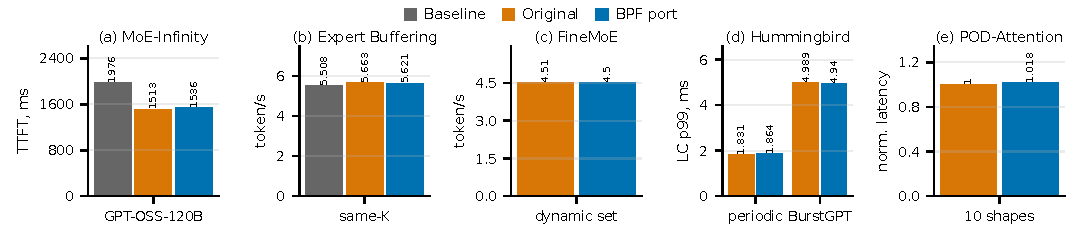
\includegraphics[width=\textwidth]{img/results-raw/revision/matched-port-panels.pdf}
\caption{Matched reimplementations of published policies on RTX~5090: each panel pairs the original implementation with the \sys{} port of the same policy. Higher is better for token/s, lower for latency.}
% RTX~5090 上对已发表策略的匹配重实现：每个子图将原始实现与同一策略的 \sys{} 移植版配对。token/s 越高越好，延迟越低越好。
\label{fig:matched-ports}
\end{figure*}

\paragraph{Methodology}
% 方法
Each comparison pairs a native implementation with a \sys{} port of the same policy on the same workload and executor, on RTX~5090 (driver 575.57.08) with exclusive GPU access and repeated randomized trials; a paper-described component reimplementation is distinguished from an upstream artifact below.
% 每组对比在相同工作负载和执行器上，将原生实现与同一策略的 \sys{} 移植版配对，在 RTX~5090（驱动 575.57.08）上以独占 GPU 和重复随机试验运行；下文区分按论文描述复刻的组件与上游工件。
Every configuration passes numerical correctness checks with the policy verifiably executing; we report medians with paired bootstrap intervals.
% 每种配置都通过数值正确性检查且策略可验证地执行；报告中位数及配对 bootstrap 区间。

\paragraph{MoE-Infinity (expert offloading)}
% MoE-Infinity（专家卸载）
We port MoE-Infinity's~\cite{xue2025moeinfinity} activation-aware prediction, prefetch ranking, and score-based eviction to host-JIT \sys{} selectors sharing the same GPT-OSS-120B frontend.
% 我们将 MoE-Infinity~\cite{xue2025moeinfinity} 的激活感知预测、预取排序和基于分数的驱逐移植到共享同一 GPT-OSS-120B 前端的 \sys{} 主机 JIT 选择器。
Across five repeated runs, baseline, native, and \sys{} achieve 11.90, 11.22, and 11.19 tokens/s: the \sys{} port tracks the native policy within 0.4\% while cutting first-visible-text latency by 22.5\% relative to baseline.
% 五次重复试验下，基线、原生实现和 \sys{} 分别达到 11.90、11.22 和 11.19 token/s：\sys{} 移植版与原生策略的差距在 0.4\% 以内，同时相对基线将首个可见文本延迟降低 22.5\%。

\paragraph{XSched (preemptive scheduling)}
% XSched（抢占式调度）
We port XSched's~\cite{shen2025xsched} inter-kernel preemption: a host-JIT \sys{} program makes the bounded highest-priority-first decision while the original executor performs suspend/resume.
% 我们移植 XSched~\cite{shen2025xsched} 的内核间抢占：主机 JIT 的 \sys{} 程序做出有界的最高优先级优先决策，由原始执行器执行挂起/恢复。
LC submission-to-first-CTA p99 is 76.9~s native, 27.0~s with XSched, and 27.3~s with the \sys{} port (paired difference $+0.29$~s, CI $[-0.11,+0.64]$), with BE throughput unchanged.
% LC 提交到首个 CTA 的 p99：原生 76.9 秒，XSched 27.0 秒，\sys{} 移植版 27.3 秒（配对差 $+0.29$ 秒，CI $[-0.11,+0.64]$），BE 吞吐量不变。

\paragraph{GPREEMPT (priority timeslicing)}
% GPREEMPT（优先级时间片）
Under continuous background load, the GPREEMPT~\cite{fan2025gpreempt} policy reduces LC response p99 from 1.796~ms (native) to 1.615~ms (original C) and 1.610~ms (\sys{}), at about 9\% background-throughput cost in both implementations; the \sys{} port differs from the original C by $-1.3\%$ (CI $[-4.2\%,+0.5\%]$).
% 在连续后台负载下，GPREEMPT~\cite{fan2025gpreempt} 策略将 LC 响应 p99 从 1.796 毫秒（原生）降至 1.615 毫秒（原始 C 实现）和 1.610 毫秒（\sys{}），两种实现都付出约 9\% 的后台吞吐量代价；\sys{} 移植版与原始 C 的差异为 $-1.3\%$（CI $[-4.2\%,+0.5\%]$）。
A knee sweep brackets full foreground coverage at 625 requests/s.
% 拐点扫描在每秒 625 个请求处界定了前台全覆盖的范围。

\paragraph{Expert Buffering (expert residency)}
% Expert Buffering（专家驻留）
Porting Expert Buffering's~\cite{huang2023towards} inactive-first hot-expert residency to the same executor improves throughput over a fixed-$K$ FIFO baseline by 2.6\% (native) and 1.8\% (\sys{}), with identical residency decisions and 12.9\% less copy payload; the \sys{} path costs 0.7\% relative to the native policy.
% 将 Expert Buffering~\cite{huang2023towards} 的非活跃优先热专家驻留策略移植到同一执行器，相比固定 $K$ FIFO 基线吞吐量提升 2.6\%（原生）和 1.8\%（\sys{}），驻留决策完全一致且拷贝负载减少 12.9\%；\sys{} 路径相对原生策略的代价为 0.7\%。

\paragraph{FineMoE (dynamic expert sets)}
% FineMoE（动态专家集）
For FineMoE's~\cite{yu2026finemoe} dynamic expert-set selection, the demand-only baseline disables speculative prefetch; the all-positive ablation instead prefetches every positive prediction.
% 对 FineMoE~\cite{yu2026finemoe} 的动态专家集选择，按需基线关闭推测预取；全正例消融则预取所有正预测。
Across five blocks, demand-only, all-positive, native C, and \sys{} achieve median throughput of 5.171, 3.623, 4.499, and 4.514 tokens/s.
% 五组实验中，按需、全正例、原生 C 和 \sys{} 的吞吐中位数分别为 5.171、3.623、4.499 和 4.514 token/s。
The \sys{} policy reduces evicted-unused speculative payload by 60.4\% and improves paired throughput by 24.6\% over all-positive, but loses 12.6\% throughput against demand-only: less waste does not guarantee a net prefetch benefit.
% \sys{} 策略相对全正例减少了 60.4\% 的未使用即被驱逐的推测负载，配对吞吐提高 24.6\%，但相对按需基线吞吐下降 12.6\%：浪费减少不保证预取的净收益。
The BPF/native paired throughput difference is $+0.21\%$ (95\% CI $[-0.17\%,+0.52\%]$), with no detected directional mechanism effect.
% BPF/原生的配对吞吐差异为 $+0.21\%$（95\% CI $[-0.17\%,+0.52\%]$），未检测到明确方向的机制效应。

\paragraph{Hummingbird (idle admission)}
% Hummingbird（空闲准入）
We port Hummingbird's~\cite{hu2026hummingbird} idle-interval admission component to both a C implementation and a host-JIT \sys{} program on the same DNN frontend, under periodic and BurstGPT arrivals.
% 我们将 Hummingbird~\cite{hu2026hummingbird} 的空闲区间准入组件在同一 DNN 前端上分别实现为 C 版本和主机 JIT 的 \sys{} 程序，覆盖周期性和 BurstGPT 两种到达模式。
Relative to default scheduling, idle admission lowers median LC response p99 from 1.980 to 1.831/1.864~ms (C/\sys{}) for periodic arrivals, and from 5.436 to 4.989/4.940~ms for BurstGPT arrivals.
% 相比默认调度，空闲准入将周期性到达的 LC 响应 p99 中位数从 1.980 降至 1.831/1.864 毫秒（C/\sys{}），将 BurstGPT 到达的相应值从 5.436 降至 4.989/4.940 毫秒。
This foreground benefit costs background throughput: both ports deliver about 133 requests/s versus 179 for default scheduling, and lose 19--20\% to the fixed-GPREEMPT control in paired comparisons.
% 这一前台收益付出了后台吞吐代价：两个移植版约为每秒 133 个请求，默认调度约为 179；相对固定 GPREEMPT 对照，配对吞吐下降 19--20\%。
These are conservative reimplementations of the idle-admission component, not the authors' complete scheduler; similar C/BPF goodput does not establish identical foreground protection.
% 这些是空闲准入组件的保守重实现，而非作者的完整调度器；相近的 C/BPF 有效吞吐不能证明前台保护相同。

\paragraph{POD-Attention (device-side selection)}
% POD-Attention（设备端选择）
A device-BPF selector implements POD-Attention's~\cite{kamath2025pod} proportional SM-local task choice; the five-arm comparison includes non-fused FlashAttention serial and two-stream baselines, upstream POD inline selection, a CUDA adapter, and the BPF adapter across ten shapes and five blocks.
% 设备端 BPF 选择器实现 POD-Attention~\cite{kamath2025pod} 按比例的 SM 本地任务选择；五臂比较覆盖未融合的 FlashAttention 串行和双流基线、上游 POD 内联选择、CUDA 适配器和 BPF 适配器，共十种形状、五组实验。
BPF beats the two-stream baseline in seven shapes, not all: for Llama decode batch 128, baseline/CUDA/BPF operator latency is 5.360/4.322/4.344~ms, whereas batch 32 gives 3.303/3.460/3.494~ms.
% BPF 在七种而非全部形状上优于双流基线：Llama 解码批量 128 时基线/CUDA/BPF 算子延迟为 5.360/4.322/4.344 毫秒，批量 32 时则为 3.303/3.460/3.494 毫秒。
Fusion gains belong to POD's policy/operator; the BPF/CUDA paired latency cost is 0.51--1.18\% in nine shapes, with a 0.44\% reduction in the remaining shape.
% 融合收益来自 POD 的策略/算子；九种形状中 BPF/CUDA 配对延迟代价为 0.51--1.18\%，剩余一种降低 0.44\%。
The separate batch-32 setup-decomposition study measures a 1.78\% operator cost, not a ten-shape average, and reports 271~s of BPF startup before the first Python statement, outside operator timing.
% 独立的批量 32 启动分解实验测得 1.78\% 算子代价，而非十种形状的平均值，并记录了首条 Python 语句之前 271 秒的 BPF 启动时间，不计入算子计时。

\paragraph{Mechanism cost}
% 机制代价
Across the matched ports, executing the same policy through \sys{} costs 0.7--3.3\%: 0.7\% for Expert Buffering, 1.8\% for POD-Attention's device selector, and 3.2\% for a kernel-verified UVM no-prefetch policy measured over fifteen paired fault-path runs.
% 在所有匹配移植中，通过 \sys{} 执行相同策略的代价为 0.7--3.3\%：Expert Buffering 为 0.7\%，POD-Attention 设备端选择器为 1.8\%，经内核验证的 UVM 无预取策略在十五次配对缺页路径运行上测得 3.2\%。
The headline improvements in RQ1 are therefore policy gains, obtainable through a safe, dynamic, and full-stack mechanism at single-digit cost.
% 因此，RQ1 中的头条提升是策略收益，可以通过一个安全、动态、全栈的机制以个位数的代价获得。

\paragraph{Agent-discovered policies}
% 智能体发现的策略
Beyond reproducing published policies, the mechanism enables policies that no existing system implements.
% 除了复现已发表的策略，该机制还使能了任何现有系统都未实现的策略。
In the MoE study (\S\ref{sec:eval}), device-side tracing led the agent to a stride-prefetch policy aligned with per-layer expert weight layout combined with LFU eviction that protects shared layers; in the KV-cache study, the agent differentiated prefetch by region type (stride for weights, sequential for KV-cache) under a PCIe-utilization budget, avoiding the mutual thrashing that a uniform policy causes.
% 在 MoE 研究（\S\ref{sec:eval}）中，设备端追踪引导智能体得出与每层专家权重布局对齐的步长预取策略，并结合保护共享层的 LFU 驱逐；在 KV-cache 研究中，智能体在 PCIe 利用率预算下按区域类型区分预取（权重用步长、KV-cache 用顺序），避免了统一策略导致的相互抖动。
These policies depend on cross-layer observations---device-side access patterns driving host-side migration---that framework-level mechanisms cannot express.
% 这些策略依赖跨层观测——由设备端访问模式驱动主机端迁移——这是框架层机制无法表达的。
